
%(BEGIN_QUESTION)
% Copyright 2011, Tony R. Kuphaldt, released under the Creative Commons Attribution License (v 1.0)
% This means you may do almost anything with this work of mine, so long as you give me proper credit

The following variable-speed motor drive receives a variable DC voltage from a potentiometer as a speed-command signal from a human operator.  In this case, the potentiometer's full range commands the motor to spin from 0 RPM to 1800 RPM (the wiper here is drawn in a position nearer 100\% speed:

$$\includegraphics[width=15.5cm]{i03289x01.eps}$$

One day the operations manager approaches you to request you modify this speed-command system so that the operators cannot call for a speed less than 100 RPM or greater than 1670 RPM.  You consult the manual for the motor drive, and are surprised to find it lacks this sort of capability: a resistance input of 0 to 10 k$\Omega$ will {\it only} translate to a speed range of 0 to 1800 RPM.  This means you must figure out a way to set the adjustable speed range limits externally to the drive (i.e. by limiting the range of the potentiometer's resistance adjustment).

You know you cannot mechanically limit the turning of the potentiometer knob, but you can connect fixed-value resistors to the potentiometer to {\it electrically} limit its range, so that full clockwise will only command the drive to go as high as 1670 RPM, and full-counterclockwise will only command the drive to go as low as 100 RPM.

\vskip 10pt

Modify this diagram to include any necessary fixed-value resistors, and also calculate their necessary values.

\vfil 

\underbar{file i03289}
\eject
%(END_QUESTION)





%(BEGIN_ANSWER)

This is a graded question -- no answers or hints given!

%(END_ANSWER)





%(BEGIN_NOTES)

This VFD receives a 0-10 VDC signal from the potentiometer to tell it to spin between 0 and 1800 RPM.  Therefore, in order to limit the speed range from 100 RPM to 1670 RPM, we must limit the voltage signal to a range of 0.556 VDC to 9.278 VDC (i.e. a voltage-division ratio of 5.56\% to 92.78\%).

\vskip 10pt

Placing two resistors in series with the potentiometer -- one on the positive side and one on the negative side -- will have the desired effect of limiting the pot's adjustment range to any values we choose.  The task we are faced with now is how to select those two resistor values to suit our needs in this scenario.

\vskip 10pt

Recall from your study of systems of linear equations that in order to solve for multiple unknowns we must have multiple equations to work with.  Therefore, in order to solve for the values of {\it two} resistors, we must have {\it two} equations describing the resistor network.  We may write two equations showing the division ratio of the potentiometer circuit, one with the potentiometer at the minimum-speed position (100 RPM), and the other with the potentiometer at the maximum-speed position (1670 RPM).

\vskip 10pt

Simultaneous equations for voltage divider resistor solution (resistor on low side being $x$ and resistor on high side being $y$):

$${x \over {x + y + 10000}} = {100 \over 1800} \hskip 50pt {{x + 10000} \over {x + y + 10000}} = {1670 \over 1800}$$

At this point, we use algebra to solve for $x$ and $y$:

$$\includegraphics[width=15.5cm]{i03289x02.eps}$$

%INDEX% Mathematics review: simultaneous equations

%(END_NOTES)


